\section{Identification of Multiple Scattering Events }
\label{secPosRecCuts}

The standard approach to identify a multiple scatter interaction is to search for several S2 peaks in an event waveform. However, when a particle interacts in multiples places of the target volume, which are very close in $Z$, the resolution of the peak finder (Section~\ref{secPositionResolution}) does not allow to identify separate S2 peaks. Hence, based only on this waveform, such events would be wrongly identified as single scatters, leading to a possible false WIMP signal. Identification of multiple scattering events is performed based on the S2 light pattern. Two cuts have been developed for this purpose.

For each S2 peak, a $\chi^{2}$ value is computed by comparing the light pattern on the top array in the measured data to the simulated pattern, which corresponds to the reconstructed position. The reduced $\chi^{2}$ has been calculated taking into account the number of the PMTs in the top array. The distribution of this parameter for nuclear recoils from an $^{241}$Am-Be calibration is shown in Fig.~\ref{figPosRecCuts_1}, together with the possible cuts and their acceptance. The events with large reduced $\chi^{2}$ are likely not a single interaction.

\begin{figure}[!b]
\centering
\subfigure[]{
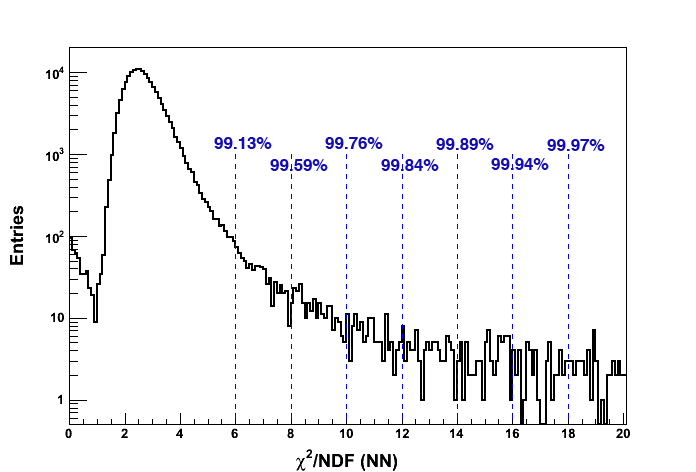
\includegraphics[height=0.375\linewidth]{plots/PosRecCuts/CHInn_OnlyQualityCuts_WithLines_wide_WithNumbers.png}
\label{figPosRecCuts_1}}
\subfigure[]{
\includegraphics[height=0.375\linewidth]{plots/PosRecCuts/H2_Xdif_COLZ_Ncuts1_WithCutLinesandAcceptance.png}
\label{figPosRecCuts_2}}
\caption[The $\chi^{2}$ value for the positions reconstructed with the NN algorithm and Euclidean distance between the points reconstructed with different algorithms for $^{241}$Am-Be calibration data]{The $\chi^{2}$ value for the positions reconstructed with the NN algorithm (a) and Euclidean distance between the points reconstructed with different algorithms (b) for $^{241}$Am-Be calibration data. The numbers indicate the nuclear recoil acceptance of possible cuts.}
\label{figPosRecCuts}
\end{figure}

Even though the NN algorithm has been used for the `standard' XENON100 data analysis~\cite{xe100-run08}, the information from the other two algorithms can be used to ensure the quality of the position reconstruction. As it has been shown in Fig.~\ref{figPosRecCo60}, the positions reconstructed with the $\chi^{2}$-minimization and SVM algorithms are in relatively good agreement with the NN reconstruction. In order to quantify how well the results agree, the Euclidean distance between the reconstructed points in $XY$ plane can be calculated for both algorithm pairs:

\begin{equation}
\label{eqPosRec_1}
D_{\mathrm{NN-SVM}} = \sqrt{(X_{\mathrm{NN}}-X_{\mathrm{SVM}})^{2} + (Y_{\mathrm{NN}}-Y_{\mathrm{SVM}})^{2}},
\end{equation}

\begin{equation}
\label{eqPosRec_2}
D_{\mathrm{NN}-\chi^{2}} = \sqrt{(X_{\mathrm{NN}}-X_{\chi^{2}})^{2} + (Y_{\mathrm{NN}}-Y_{\chi^{2}})^{2}}.
\end{equation}

The computed $D$s are shown in Fig.~\ref{figPosRecCuts_2}. For most of the events the distance between the reconstructed points is within a few mm. However, there are outliers, for which the distance is 1~cm and more, which could be cut to ensure the position reconstruction quality.

The Euclidean distance for the algorithm pairs calculated with formulas (\ref{eqPosRec_1}) and (\ref{eqPosRec_2}) can be combined into a one-dimensional radial cut (`combined Euclidean distance'). The possible cuts and the corresponding acceptance are shown by the circular lines in Fig.~\ref{figPosRecCuts_2}.

\begin{equation}
D = \sqrt{D_{\mathrm{NN}-\mathrm{SVM}}^{2} + D_{\mathrm{NN}-\chi^2}^{2}}.
\end{equation}

Figure~\ref{figPosRecCutsResults_1} shows the correlation between the two discrimination parameters introduced above, based on the reduced $\chi^{2}$ value for the positions reconstructed with the NN algorithm and the Euclidean distance between the points reconstructed with NN, SVM, and $\chi^{2}$-minimization algorithms. 
The red lines show the chosen cuts, with a total nuclear recoil acceptance of 98\%. 

An example of a light pattern for an event which is removed with the described cuts is presented in Fig.~\ref{figPosRecCutsResults_2}. It clearly shows two interaction spots at distant places in the $XY$ plane, and confirms that this event is most likely a multiple interaction in the target volume. The position of the event is reconstructed as the weighted average, in the middle of the light spots, which results in a large $\chi^{2}$ value.

\begin{figure}[!h]
\centering
\subfigure[]{
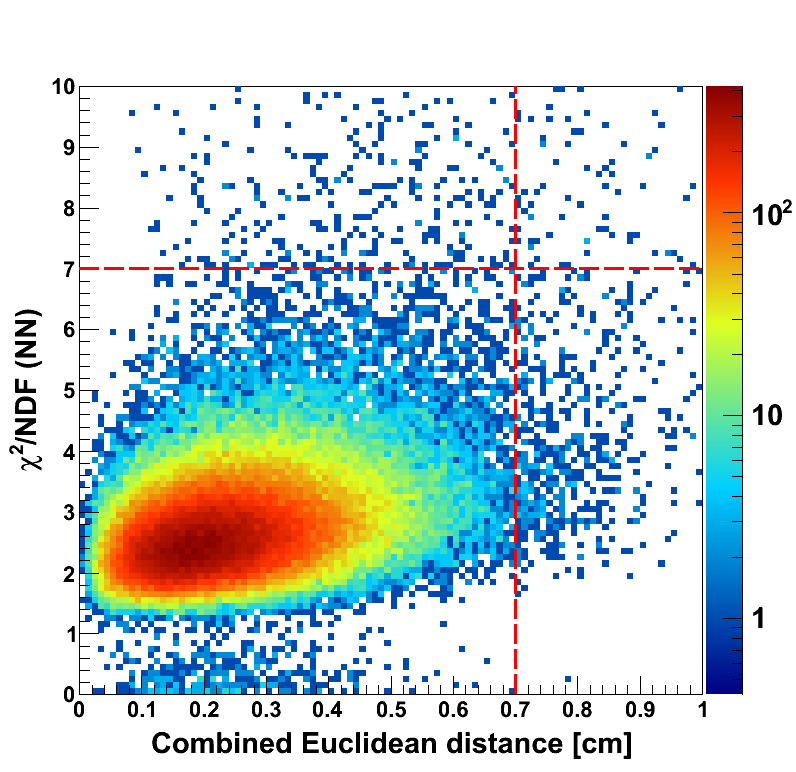
\includegraphics[height=0.4\linewidth]{plots/PosRecCuts/XdifChi_AmBe_Ncuts1.png}
\label{figPosRecCutsResults_1}}
\subfigure[]{
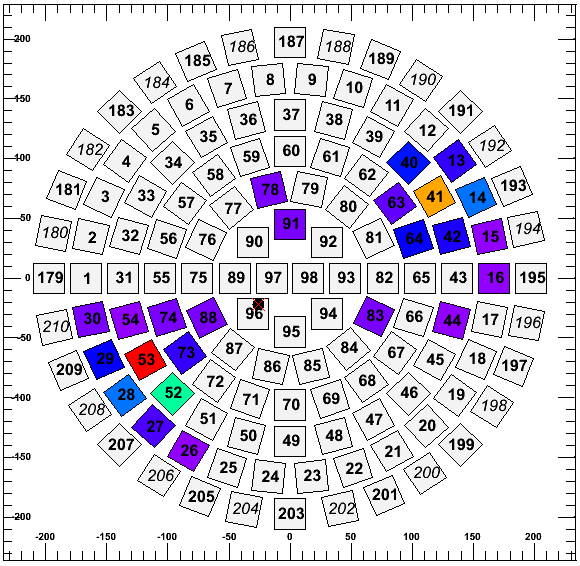
\includegraphics[height=0.39\linewidth]{plots/PosRecCuts/b_6.png}
\label{figPosRecCutsResults_2}}
\caption[Discrimination parameters based on the $\chi^{2}$ and the Euclidean distance, and an example of light pattern for a multiple scattering event]{(a) - discrimination parameters based on the reduced $\chi^{2}$ value for the positions reconstructed with the NN algorithm and Euclidean distance between the points reconstructed with NN, SVM and $\chi^{2}$-minimization algorithms. The lines show the cuts chosen for the XENON100 data analysis~\cite{xe100-run08} with the total nuclear recoil acceptance of 98\%. (b) - an example of a light pattern for an events with multiple interactions close in $Z$. The black circle with a red cross shows the wrongly reconstructed position. This event is removed with the cuts shown in figure (a).}
\label{figPosRecCutsResults}
\end{figure}


